\documentclass[12pt,a4paper]{article}
\usepackage{setspace} \onehalfspacing
\usepackage[top = 1in, bottom = 1in, left = 1in, right = 1in]{geometry}
\usepackage[utf8]{inputenc}
\usepackage{amsmath}
\usepackage{amsfonts}
\usepackage{amssymb}
\usepackage{amsthm}
\usepackage{graphicx}
\usepackage{natbib}
\usepackage{caption}
\usepackage{subcaption}
\usepackage{float}
\usepackage{pdflscape}
\usepackage{booktabs}
\usepackage{dcolumn}
\usepackage{pdflscape}
% \usepackage{hyperref}
\usepackage[hyphens]{url}
\usepackage{enumitem}
\usepackage[table]{xcolor}
\usepackage{authblk}
\usepackage{appendix}
\usepackage{titletoc}
\usepackage{fancyhdr}
\usepackage{hyperref}

\bibliographystyle{apsr}

\newcommand{\note}{\textcolor{blue}}

\title{A partisan affair: Mapping patronage in municipal bureaucracies of Brazil}
\author{Galileu Kim}
\affil{Princeton University}

\begin{document}

\maketitle

\abstract{How extensive is patronage in Brazil? What are the differences in observables between partisan affiliates and non-partisan members? Leveraging a novel dataset of partisan affiliation and employment data on every municipal bureaucrat in Brazil, I find that party members are more likely to be overcompensated than their peers, concentrating in areas of executive leadership, while being less educated than their peers. In addition, their employment spells tend to be more durable over time, leading to the build-up of party members in the bureaucracy over time. These findings provide raise important questions regarding the nature of patronage, party building and its consequences for local bureaucracies.}

\newpage

\section{Introduction}
\label{sec:intro}

Who benefits from patronage? And what are its consequences for local administration? 

Literature on patronage and selection: \citet{robinson2013political}. Extant literature on selection of public officials have primarily focused on who becomes a politician \citet{dal2017becomes}. There remains unanswered questions regarding who enters the bureaucracy, what types of employment they held, and what are the differential compensations among public officials.

Empirical research on allocation of public sector jobs has consistently found that politically motivated allocation of public sector jobs is an important determinant of public employment in the developed and developing world \citep{finan2017personnel}. In the United States, appointments to the federal bureaucracy involve considerations of party loyalty and ideological alignment with the president \citep{lewis2010politics, hollibaugh2014presidents}. In Brazil, whether it be at the presidential \citep{pracca2011political} or at the municipal level \citep{colonnelli2018patronage,brollo2017victor}, politicians have discretion over bureaucratic appointments and frequently use these to further their political goals.

A set of explanations have been proposed to explain the determinants of this allocation, whether it be to reduce frictions in policy implementation due to ideological divergence \citep{krause2016experiential}, exploit the benefits of strong ties \citep{toral2019benefits} or to reward followers for campaign contributions \citep{colonnelli2018patronage}. These findings have provided important insights into the drivers of patronage appointments into employment in the public sector. Yet as important as the drivers of public sector appointment are the characteristics of those entering the bureaucracy \citep{finan2015personnel}. Who becomes a bureaucrat? Are political appointees systematically different from their non-partisan counterparts? And where, within the bureaucracy, do these patronage appointees go?

In this paper, I focus on party membership as a determinant of not only whether or not individuals enter into public sector employment, but the type of employment they receive. In particular, using a rich panel data set of all public sector workers, I identify the party membership of all municipal bureaucrats in Brazil to provide a novel set of empirical findings: 1) the pre-bureaucracy characteristics of public sector workers, 2) employment trajectories within the bureaucracy and 3) post-public sector employment of party members. This complete revolving-door of party and non-party members provide a unique frame-by-frame evolution of the employment trajectories of pre- and post-bureaucrats in a developing world context.

The main finding is that patronage primarily benefits a local economic elite, accruing to the richest formal sector workers and allocating them into the best-paying jobs in the municipal bureaucracy. These higher compensation structures are not commensurate to skills on a set of observable qualifications, such as education level and work experience, suggesting that these benefits accrue from channels other than individual skills. Additionally, party members accumulate jobs at higher levels of government such as executive leadership and administration, which are better compensated, as well as benefiting from longer income streams due to privileged access to tenured contracts.

These findings suggest that, overall, patronage does not necessarily accrue to poor voters, contrary to theoretical and empirical findings in studies of clientelism in the developing world \citep{stokes2013brokers}. A different logic seems to be at play. Patronage to party loyalists can be used strategically as a mean of securing control over the bureaucracy -- through tenured contracts -- as well as securing buy-in from wealthy patrons or notables in the local economy, consistent with empirical findings by \citet{colonnelli2018patronage}. Patronage therefore can serve a crucial role in securing access to economic resources through wealthy patrons, which in turn can be allocated to finance campaigns and other exercises in party building.

This paper contributes to literature on clientelism that outlines the political logic of patronage allocations. The contribution is twofold: 1) first, I find that patronage is a patron-elite game, generating a form of patronage that is distinct from the politician-voter nexus that has been traditionally the focus of extant literature on clientelism \citet{stokes2013brokers, diaz2016political} and 2) I find that the benefits of patronage go beyond simply an electoral pay-off. Instead, what patronage accomplishes is securing access to economic resources that can be tapped into once employment is offered to wealthy patrons, similar in spirit to the theoretical findings by \citet{robinson2013political}. Patronage binds parties and patrons, in effect capturing the benefits of public sector employment to finance efforts towards party-building.

The paper is structured as follows. Section \ref{sec:context} provides context for the data and the hiring process for local bureaucracies, while section \ref{sec:descriptive} provides some descirptive statistics outlining the differences between partisan and non-partisan members. Section \ref{sec:empirical} outlines the empirical strategy. Section \ref{sec:conclusion} concludes.

\section{Context and Data}
\label{sec:context}

\subsection{Brazilian municipal government}

Brazil is a federal republic comprised of 26 states and over 5500 municipalities. Each municipality is headed by a mayor and city councilors (\emph{vereadores}). Local officials are elected for a four-year term, with reelection. Each local election takes place at the same time, in October, with the new administration taking office in January of the following year. With decentralization embedded in the enactment of a new constitution in 1988, local municipalities were given large autonomy with respect to public services such as education and healthcare, as well as building an administrative infrastructure to oversee its daily operations \citep{souza2017modernizaccao}. 

Municipal budgets are financed with a mix of federal transfers and local revenues. Smaller municipalities tend to rely on federal transfers, which are subject to oversight by higher levels of government, either federal or state, but in practice are under large discretion by municipal governments. The past two decades have seen a growing share of expenditures social service concentrated by municipalities, which has led to expansion in access to and the quality of local services \citep{arretche2015trajetorias}. Additionally, laws and regulations concerning local economies and society are largely autonomous and instituted by the mayor's office, subject to revision and approval by the local city council \citep{brelaz2013processo}.

Finally, it municipalities are in their vast majority quite small, with approximately 90 percent of municipalities having a population of less than 50 thousand people. In contrast, the 27 state capitals (including Bras\'{i}lia) concentrate over 23 percent of the Brazilian population.\footnote{See coverage \href{https://www.google.com/search?q=tamanho+municipio+brasil+poulacao&source=lmns&hl=en&sa=X&ved=2ahUKEwjyiLjLh6buAhXFn-AKHbzEBxAQ_AUoAHoECAEQAA}{here}.} This largely uneven concentration of the Brazilian population across its municipal governments, as well as the prevalence of small, poorer municipalities, has led observants to conclude that municipal politics is often characterized by clientelism, with local political elites concentrating power through the strategic use of public resources \citep{leal2012coronelismo}.

\subsection{Municipal employment and patronage in Brazil}

Municipal employment in Brazil is under local jurisdiction, with personnel appointments under the exclusive authority of the executive branch. Salaries, contract modalities and terminations are also under municipal jurisdiction. There are multiple forms of contract available, a permanent contract (\emph{estatut\'{a}rio}), a regular contract (\emph{CLT}) and temporary hires. Personnel expenditures cannot exceed a ceiling of 60 percent of the local budget, but as long as the ceiling is not exceeded, other levels of government cannot interfere with local personnel decisions.

There are no civil service laws regulating municipal employment. With the exception of permanent contracts, municipal employees are subject to the same labor laws as private sector workers. The lack of a civil service system at the local level has been the subject of extensive research \citep{souza2004governos}, and the high turnover that are associated with municipal employment have been widely documented \citep{akhtari2017political}. Labor unions do exist, in particular in the educational sector, but these are regional in focus and concentrated in metropolitan areas. According to the latest education census (\emph{Censo do Magist\'{e}rio}), approximately 11 percent of educational staff was unionized.

Municipal discretion leaves ample room for patronage, whether it be to support mayoral coalitions as outlined in the first paper of this dissertation or to reward contributors and party loyalists \citep{colonnelli2018patronage,brollo2017victor}. These politically motivated appointments are particularly prominent in high-level positions, the so called \emph{cargos de confian\,{c}a}, local ministerial positions that are both high in compensation and provide access to decisions over key public services such as transportation and health. Regarding the nexus between party membership and public sector employment, \citet{brollo2017victor} finds that party members who are politically aligned with the winning mayor are 30 percent more likely to receive public sector employment than their runner-up counterparts.

These empirical findings suggest a clear political nexus between employment into local bureaucracies and political motives in Brazilian municipalities. This paper aims to provide an extensive treatment of the differences in the observable characteristics of party members - as opposed to their non-party members.

\subsection{Partisan affiliation in Brazil}

Partisanship in Brazil is voluntary and widespread, with over 11 percent of registered voters affiliated to a party \citep{speck2015estudo}\footnote{For context, in most OECD countries party registration does not exceed 5 percent of the electorate. See \citet{biezen2014decline}.}. Registration occurs in the following sequence: a voter reports to a municipal party office, and the party officials then register the voter officially through the \emph{Tribunal Regional Eleitoral} (Regional Electoral Office). This registration is then collected and centralized by the \emph{Tribunal Superior Eleitoral} (Supreme Electoral Office) and updated accordingly. If there are overlapping registrations, former ones become annulled and are reported as irregular to local party officials. Each voter is therefore only allowed to register for a single party, without any ceilings or floors regarding the duration of this affiliation.

There is an ongoing debate on the strength of partisan ties in Brazil. On the one hand, scholars have noted that partisanship in Brazil is weak, meaning that politicians and voters do not have strong party loyalty and often ``switch'' to other parties \citep{desposato2006parties,ames2002deadlock}. On the other, some scholars have noted that party ties have grown in strength over time, in particular for leftist programmatic parties such as the PT \citep{samuels2014power,samuels2006sources}. Part of this debate owes to disagreements on how to measure party strength, whether it be testing voters' prior knowledge of party's ideological positions or if instead, it should be measured by testing whether voters issue ballots for individual candidates or their party labels -- with each one of these measures painting an opposite picture of the relative strength of party ties.

One thing is clear: party ties at the electoral level are durable, with most voters remaining affiliated to a single party for their entire life, as highlighted by figure \emph{FIGURE}. Noting that party affiliations are registered at the municipal level, this empirical fact aligns with qualitative evidence provided by \citet{palmeira1995comicios}, who notes that parties at the local level constitute political factions (\emph{grupos pol\'{i}ticos} ) with well-defined boundaries and power disputes. This relative stability of party ties at the electorate level for the minority of voters who are registered with a parties suggests a distinct dynamic tying an elite group of party members to the city hall.

\section{Data}
\label{sec:data}

\subsection{Municipal and Private Sector Employment}

Data on formal sector employment is collected by the Department of Labor in Brazil through a census instrument, \emph{RAIS}. This instrument is completed electronically by all formally registered companies regardless of workforce size or capital, subject to sanctions if evidence of misreporting is found.\footnote{See coverage and description \href{https://agenciabrasil.ebc.com.br/economia/noticia/2020-03/prazo-para-entrega-da-rais-comeca-hoje-e-vai-ate-17-de-abril}{here}.} In total, over 97 percent of companies in the formal sector are included in the \emph{RAIS}, as well as all public sector employment, including federal, state and municipal level bureaucrats. The quality of the data is subject to constant review by the Department of Labor, which relies on accurate information to calculate taxes and retirements benefits for the Brazilian workforce. 

The \emph{RAIS} data is structured as follows. Each row corresponds to a job associated to a worker, which may or may not appear more than once in the dataset -- since workers can hold multiple jobs at the same time. Each worker is tagged by a unique national id, the \emph{CPF}, which allows for following workers across sectors and over time. Additionally, the identified \emph{RAIS} contains the names and dates of birth of workers.\footnote{Access to the identified \emph{RAIS} was generously provided by the Department of Economics at Princeton University, hosted at the Industrial Relations office.} These are the unique primary keys that make possible join this dataset to other sources of data. Other studies have leveraged similar join approaches to infer employment benefits of campaign contributors \citep{colonnelli2018patronage}, as well as whether party members receive public sector employment if they belong to the same party as the winning mayor \citep{brollo2017victor}.

In contrast to these previous studies, I leverage the rich dataset of covariates that includes, \emph{inter alia}, wage compensation, education, work experience and type of contract, to estimate differential returns to compensation, outlined in greater detail in Section \ref{sec:empirical}. The richness of \emph{RAIS} allows for a complete radiography of the public sector, revealing how compensation structures are altered by their intersection with patronage dynamics. In particular, because of the panel nature of its structure, researchers can follow bureaucrats before and after their public sector employment spell, providing an unprecedently accurate depiction of the municipal revolving door.

\subsection{Partisan affiliation}

Data on partisan affiliation is detailed as well. The \emph{TSE}, the national electoral authority, collects data on all party members in the national territory, including commencement and termination dates, affiliated party, municipality and name of the registered party member, as well as their electoral title.\footnote{The data is available \href{https://filia-consulta.tse.jus.br/}{here}.} Parties are mandated by electoral law to report all party members as well as providing updated registry information throughout the year. Parties have municipal offices in which citizens may update their registry, and these party offices in turn report to the state electoral authority, which relays this information to national electoral authorities. If irregularities are found parties may be sanctioned by the \emph{TSE}.

The party affiliation data is structured as a rolling registry (\emph{fita espelho}), in which existing and expired party memberships are preserved. Each row therefore corresponds to a particular party member entry, containing the state, municipality, electoral zone and date of the registration. Additionally, the registry indicates the status of the membership, whether it is active (\emph{regular}) or canceled (\emph{cancelado/desfiliado}), as well as the date of the change in the membership status. Individual identifiers are provided, including the name and a nationally unique electoral title (\emph{t\'{i}tulo eleitoral}) that allows researchers to join names contained in the \emph{RAIS} and party affiliation data.

Note that party affiliation in Brazil is high, with over 10 percent of nationally registered voters affiliated to a political party \citep{speck2015estudo}. Partisan ties at the electorate level are stable, in contrast with more strategic party switching occurs at the political candidate level \citep{desposato2006parties}. As of 2019, the year for which party affiliation data was extracted, there were over 11 million active party affiliates, with around 5 million registries either canceled or terminated by party members.

\section{Descriptive statistics}
\label{sec:descriptive}

In this section, I provide descriptive statistics that illustrate broader patterns in the distribution of party affiliated bureaucrats at the municipal level in Brazil. Figure \ref{fig:map_pooled} illustrates the subnational distribution of party affiliation in Brazil for the year of 2015. There are a few patterns that emerge.

First, that the distribution of partisan affiliation varies significantly over the national territory, with its predominance in the Northeast, as well as in the Northern regions of the country. The Midwest and Southeast appear to have the lowest prevalence of partisan affiliation. Second, that there is wide variation with respect to the prevalence of partisanship. In particular, some municipalities are almost entirely occupied by party members, with over 60 percent of its workforce affiliated to a party. Others are largely autonomous from party members, with less than 10 percent of municipal workers affiliated to a party.

\begin{figure}[H]
    \centering
    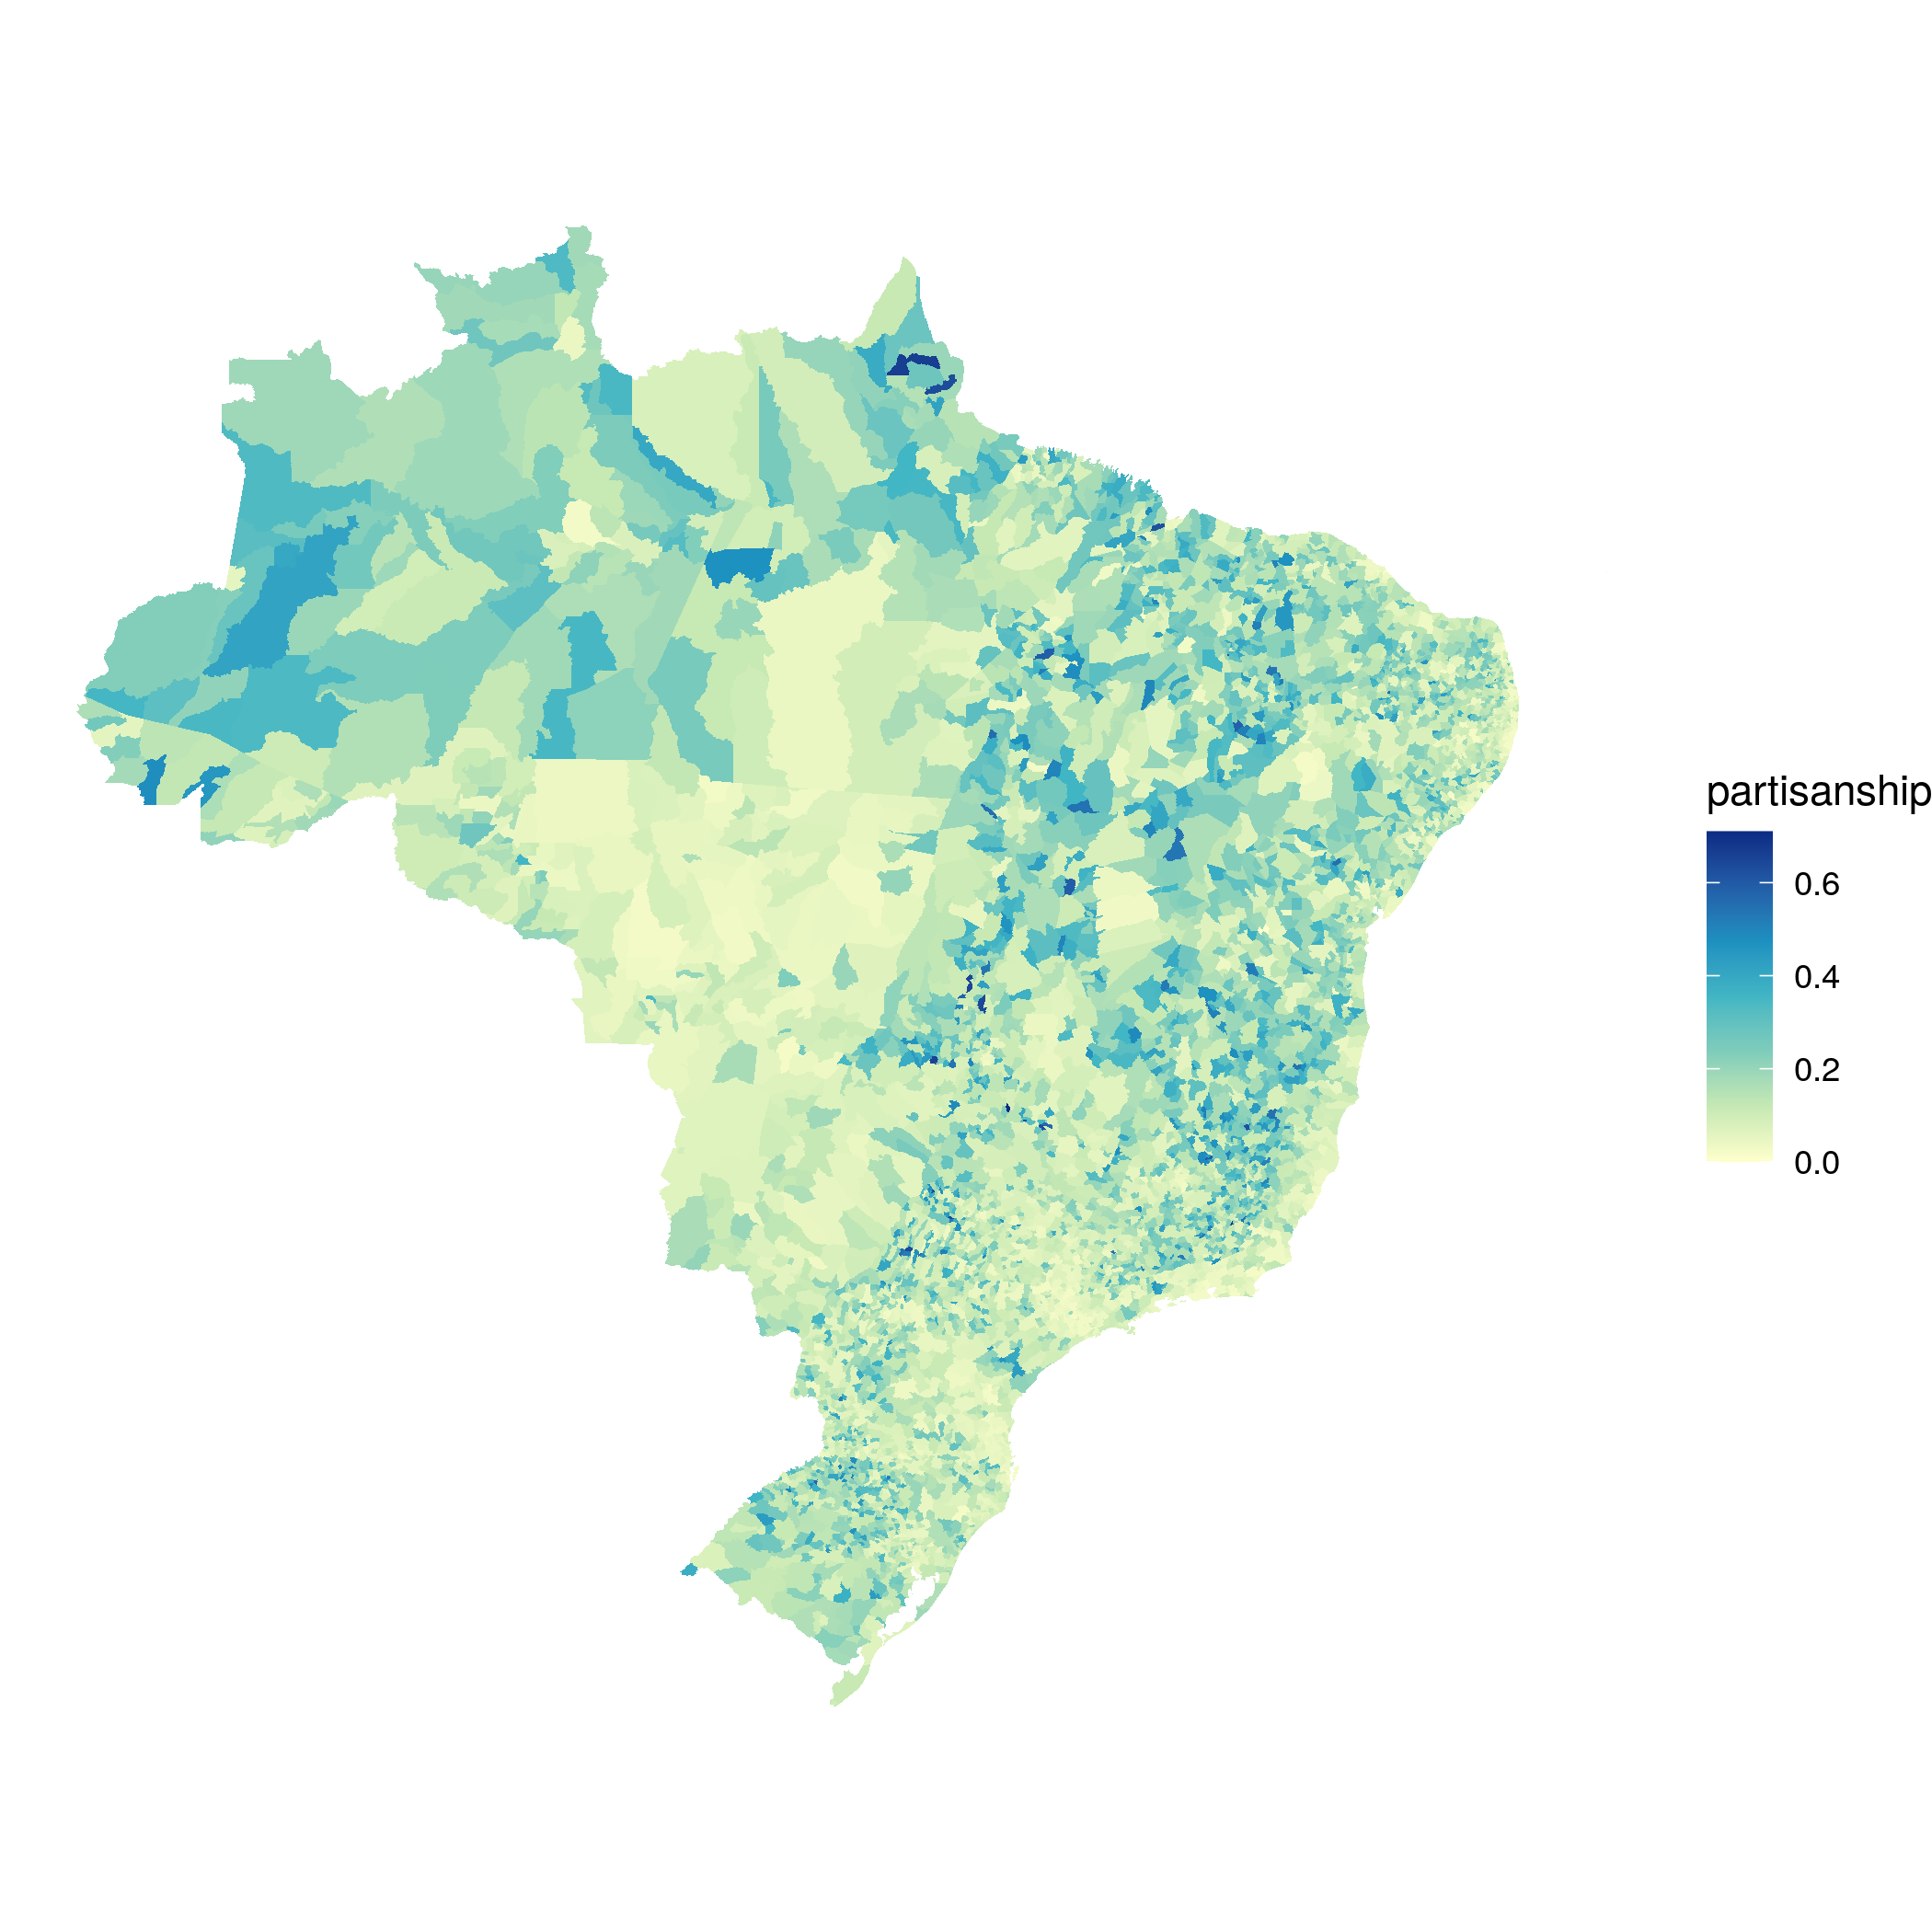
\includegraphics{figures/maps/pooled.png}
    \caption{\textbf{Proportion of party-affiliated members by municipality (2015)}. Darker colors indicate a larger degree of partisan affiliation. This visualization includes all bureaucrats, from high-level managers to service staff.}
    \label{fig:map_pooled}
\end{figure}

\section{Empirical strategy}
\label{sec:empirical}

\section{Conclusion}
\label{sec:conclusion}

\newpage

\bibliography{patronage}

\end{document}